% Chapter Template

\chapter{SCgPC and HDMR for Time-Dependent Analysis} % Main chapter title

\label{ch:timedep} % Change X to a consecutive number; for referencing this chapter elsewhere, use \ref{ChapterX}

\lhead{Chapter 9. \emph{Time-Dependent Analysis}} % Change X to a consecutive number; this is for the header on each page - perhaps a shortened title

%----------------------------------------------------------------------------------------
%	SECTION 1
%----------------------------------------------------------------------------------------

\section{Introduction}
Up to now in this work we have restricted ourselves to models with a set of single-valued responses.  One of the strengths
of the \raven{} \cite{OECDraven} framework is its innate ability to extend reduced-order models (such as the stochastic 
collocation for generalized polynomial chaos and high-density model reduction expansions) to
include time-dependent analysis.  \raven{} does this by taking snapshots in time and interpolating between them to evaluate
the reduced-order model at any time.  As part of this work we added the algorithms necessary to do this snapshot-based
time-dependent analysis for both the stochastic collocation for generalized polynomial chaos and the high-density model
reduction methods. Conveniently, no additional quadrature points are required to perform transient instead of static
uncertainty quantification using SCgPC or HDMR methods.  It should be noted, however, that adaptive SCgPC and adaptive
HDMR are not well-suited to time-dependent analysis because of the plethora of responses; effectively, there is a
full set of responses for each snapshot in time, making it difficult for the adaptive algorithms to determine the
ideal polynomials to add.

To demonstrate performance of this feature, we sought a time-dependent response with transient behavior.
Because none of the analytical models nor the \mammoth{} pincell problem have notable transient behavior, we consider
a \bison{} \cite{OECDbison} simulation of an OECD benchmak \cite{OECDbenchmark} where the performance of light-water reactor fuel 
through several power transients is analyzed.  A first pass at uncertainty quantification for this benchmark
is performed in \cite{OECDdakota}, and we use the same input variables and uncertainty distributions here.

\section{Problem Description}
The problem considered here is Case 2a defined in Chapter 2 of the benchmark report \cite{OECDbenchmark}.  It
involves several different steady-state fuel behaviors after transitioning power levels for a pressurized
water reactor fuel pin.  The \bison{} mesh used for this problem is a smeared-pellet mesh, as was also used in
\cite{OECDdakota}.  This allows the mesh to be generated directly through the \bison{} input rather than
coupling a mesh generation code to \bison{} in \raven{}.  During the simulation the pellet expands to make
contact with the cladding, and modeling persists before and after this phenomenon.  The mesh is axisymmetric
2-D in R-Z geometry, using 4290 QUAD8 finite elements or 324 thousand degrees of freedom \cite{OECDdakota}.
Because \raven{} couples with \bison{} natively, the input-output processing was handled without any need for
user involvement.

The uncertain inputs to this model are given in Table \ref{tab:oecd inps}, which is based on the data in
\cite{OECDdakota}.  The input parameters are all distributed normally, with the exception of the inlet
temperature which was instead distributed uniformly.  In addition, there were several dependent inputs in the \bison{}
input file that had to be perturbed based on the independent inputs; these are provided in Table \ref{tab:oecd deps}.
The responses of interest for this model are the following:
\begin{itemize}
  \item maximum cladding temperature (\texttt{max\_clad\_surf\_temp}),
  \item percent fission gas released (\texttt{fgr\_percent}), 
  \item elongation of the cladding, and (\texttt{max\_clad\_creep\_strain})
  \item maximum creep strain on the cladding (\texttt{clad\_elongation}).
\end{itemize}
When we use the term \emph{maximum}, we refer to the maximum value obtained from 13 axial positional along the
length of the fuel.  There is a separate maximum value for each burnup time step.

\begin{table}[htb]
  \centering
  \begin{tabular}{l l|c c}\hline
    RAVEN Name & Uncertain Parameter & Mean & Std. Dev. \\ \hline
clad\_cond  & Clad Thermal Conductivity & 16.0     &     2.5 \\
clad\_thick & Cladding Thickness        & 6.7e-4   &     8.3e-6 \\
clad\_rough & Cladding Roughness        & 5.0e-7   &     1.0e-7 \\
creep\_rate & Clad Creep Rate           & 1.0      &     0.15 \\
fuel\_cond  & Fuel Thermal Conductivity & 1.0      &     0.05 \\
fuel\_dens  & Fuel Density              & 10299.24 &    51.4962 \\
fuel\_exp   & Fuel Thermal Expansion    & 1.0e-5   &     7.5e-7 \\
fuel\_rad   & Fuel Pellet Radius        & 4.7e-3   &     3.335e-6 \\
fuel\_rough & Fuel Pellet Roughness     & 2.0e-6   &     1.6667e-7 \\
fuel\_swell & Solid Fuel Swelling       & 5.58e-5  &     5.77e-6 \\
gas\_cond   & Gas Conductivity          & 1.0      &     0.025 \\
gap\_thick  & Gap Thickness             & 9.0e-5   &     8.33e-6 \\
mass\_flux  & Mass Flux                 & 3460     &    57.67 \\
rod\_press  & Rod Fill Pressure         & 1.2e6    & 40000.0 \\
sys\_press  & System Pressure           & 1.551e7  & 51648.3 \\
sys\_power  & System Power              & 1.0      &     0.016667 \\ \hline
    RAVEN Name & Uncertain Parameter & Lower Bound & Upper Bound \\ \hline
inlet\_temp & Inlet Temperature         & 558.0    & 564.0
  \end{tabular}
  \caption{OECD Benchmark Independent Inputs}
  \label{tab:oecd inputs}
\end{table}

\begin{table}[htb]
  \centering \footnotesize
  \begin{tabular}{l|l|c}\hline
Raven Name       & Bison Path                                                 & Calculation \\\hline
clad\_inner       & {Kernals.heat\_source\_clad.inner\_diameter}                & 2*(fuel\_rad + gap\_width) \\
outer\_diam\_heat  & {Kernals.heat\_source\_clad.outer\_diameter}              & 2*(fuel\_rad + gap\_width + clad\_thick) \\
sys\_press\_cool   & {CoolantChannel.convective\_clad\_surface.inlet\_pressure}& sys\_press \\
outer\_diam\_cool  & {CoolantChannel.convective\_clad\_surface.rod\_diameter}  & 2*(fuel\_rad + gap\_width + clad\_thick) \\
porosity\_thermal & {Materials.fuel\_thermal.intial\_porosity}                 & 1 - fuel\_dens/10980 \\
fuel\_diam        & {Materials.fuel\_relocation.diameter}                      & 2*fuel\_rad \\
gap\_diam         & {Materials.fuel\_relocation.gap}                           & 2*gap\_thick \\
porosity\_sifgr   & {Materials.fission\_gas\_release.initial\_porosity}         & 1 - fuel\_dens/10980
  \end{tabular}
  \caption{OECD Benchmark Dependent Inputs}
  \label{tab:oecd deps}
\end{table}


\section{Results}
Of particular interest in this problem is analysis of sensitivity coefficients as they devolop in time.  As the
simulation progresses, there is a shift in the dominant physics behind response values.  For example, one of the more
dramatic physics transitions occurs as the fuel expands enough to make contact with the cladding.  To produce
this results, first-order Sobol using first-order polynomials were used.  While a more advanced analysis could
be performed, we found many of the realizations in the input space needed adjustments that could not realistically
be automated in order to be solved by \bison{}, such as preconditioning and executioner parameters.  Despite
the low order representation, however, there is significant physics demonstrated in the sensitivity results.

Figures \ref{fig:oecd clad temp} through \ref{fig:oecd elong} show the development of Sobol indices over the burnup
of the fuel, expressed in percent FIMA (fissions per initial metal atom).  In each plot, the power history
shape as a function of burnup is superimposed in dotted red, providing insight to some of the sensitivity
behaviors.  
Because of the large number of input parameters, we only show those parameters on each plot that
have significant impact on the response considered.  For clarity, we use a consistent scheme for coloring and
marking throughout the plots, where green is fuel parameters, black is system parameters, blue is gap
parameters, and magenta is clad parameters.  In each set of parameters, different symbols are used to
differentiate the various related inputs.  We consider each plot separately.  For reference, we also include
the burnup-dependent mean and standard deviation in Figure \ref{fig:oecd mean} and \ref{fig:oecd var}
respectively.  While we show the max centerline fuel mean and variance shapes, the max cladding temperature
follows the same shape.  In each figure, the magnitude of the values are scaled for each parameter by a factor
shown in the legend, which allows all the shapes to be seen clearly.
\begin{figure}[htb]
  \centering
  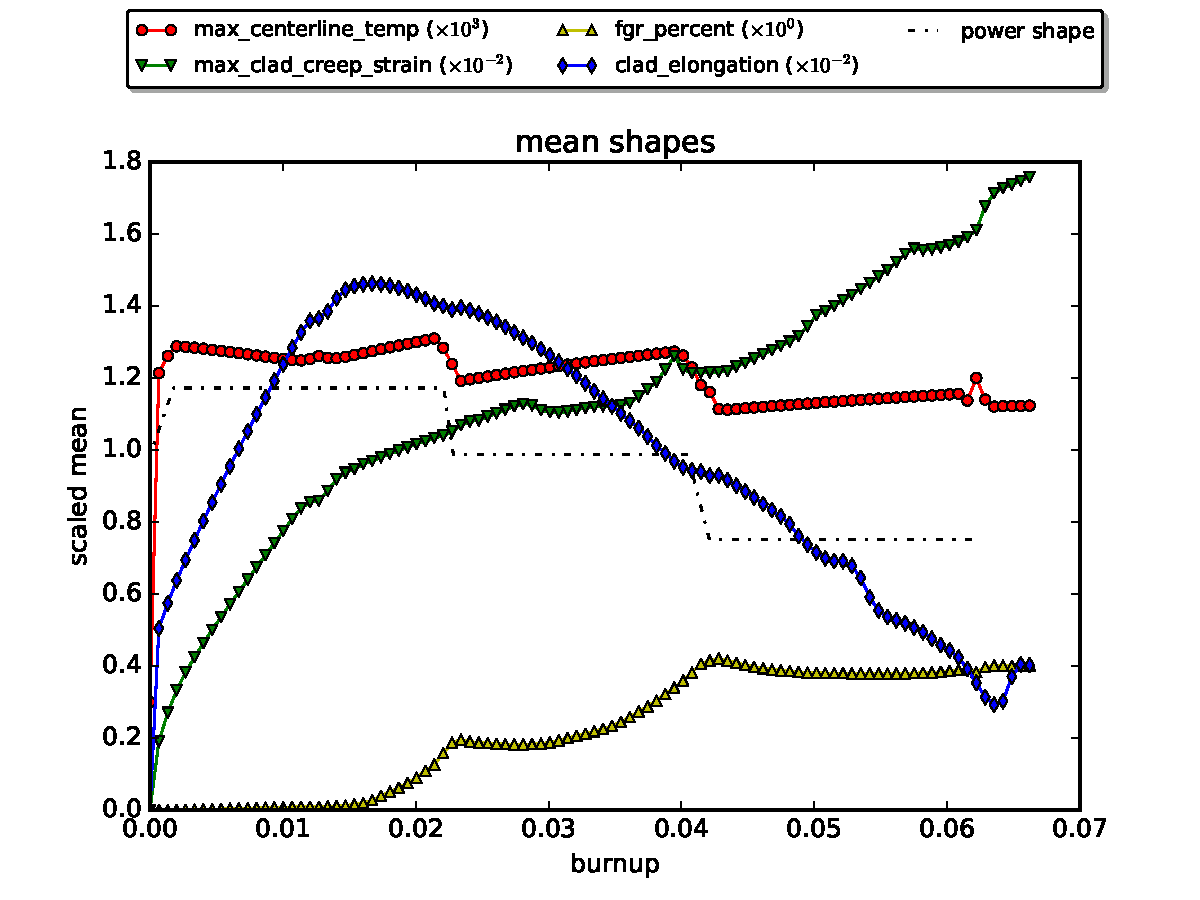
\includegraphics[width=0.7\linewidth]{oecd/meanplots}
  \caption{OECD Response Mean Values over Burnup}
  \label{fig:oecd mean}
\end{figure}
\begin{figure}[H]
  \centering
  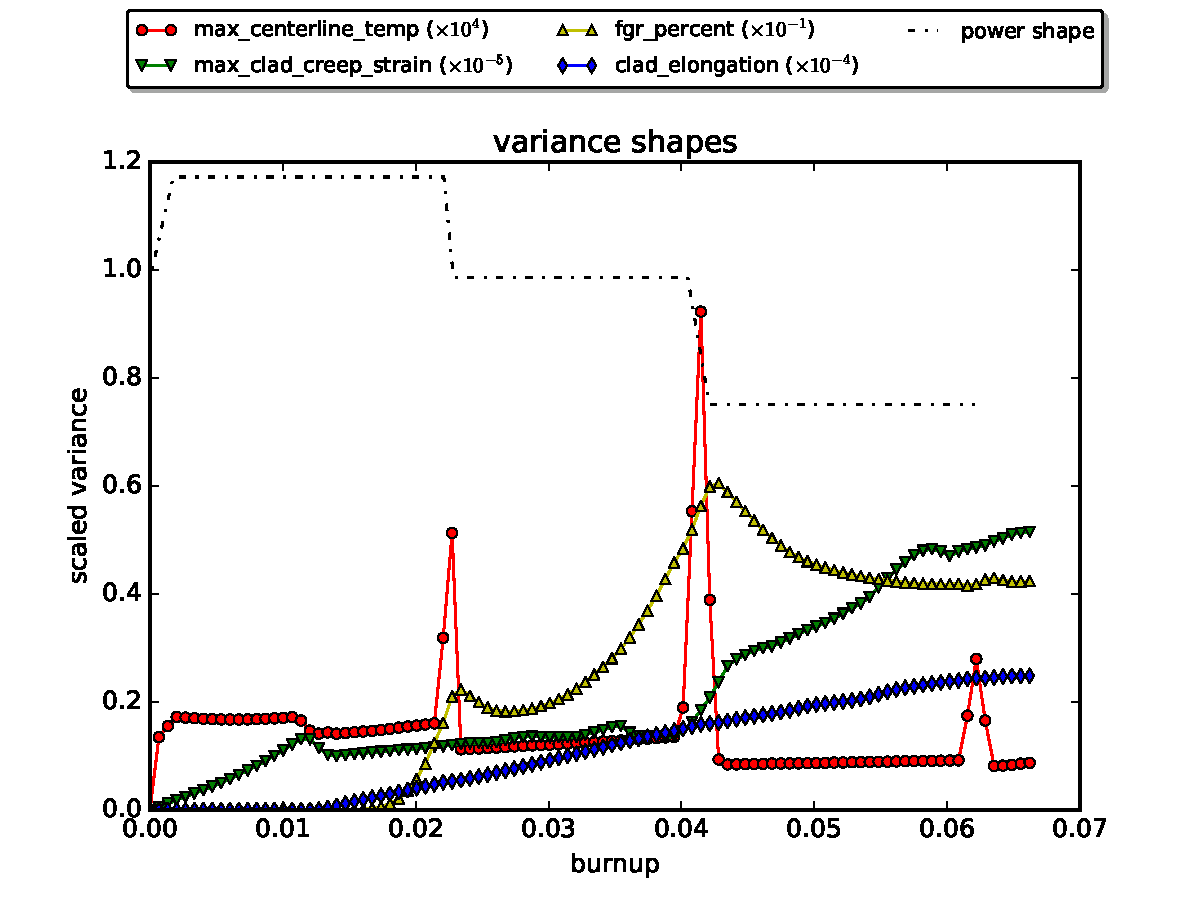
\includegraphics[width=0.7\linewidth]{oecd/varplots}
  \caption{OECD Response Variance Values over Burnup}
  \label{fig:oecd var}
\end{figure}

\subsection{Maximum Clad Surface Temperature}
One of the key design parameters for fuel in nuclear power plants, the maximum clad surface temperature is
used to quantify margin to clad melting points, at which point radioactive fuel and gas could escape into
the primary moderator loop.  Understanding the behavior of this parameter is key to the design of nuclear
fuel.
\begin{figure}[H]
  \centering
  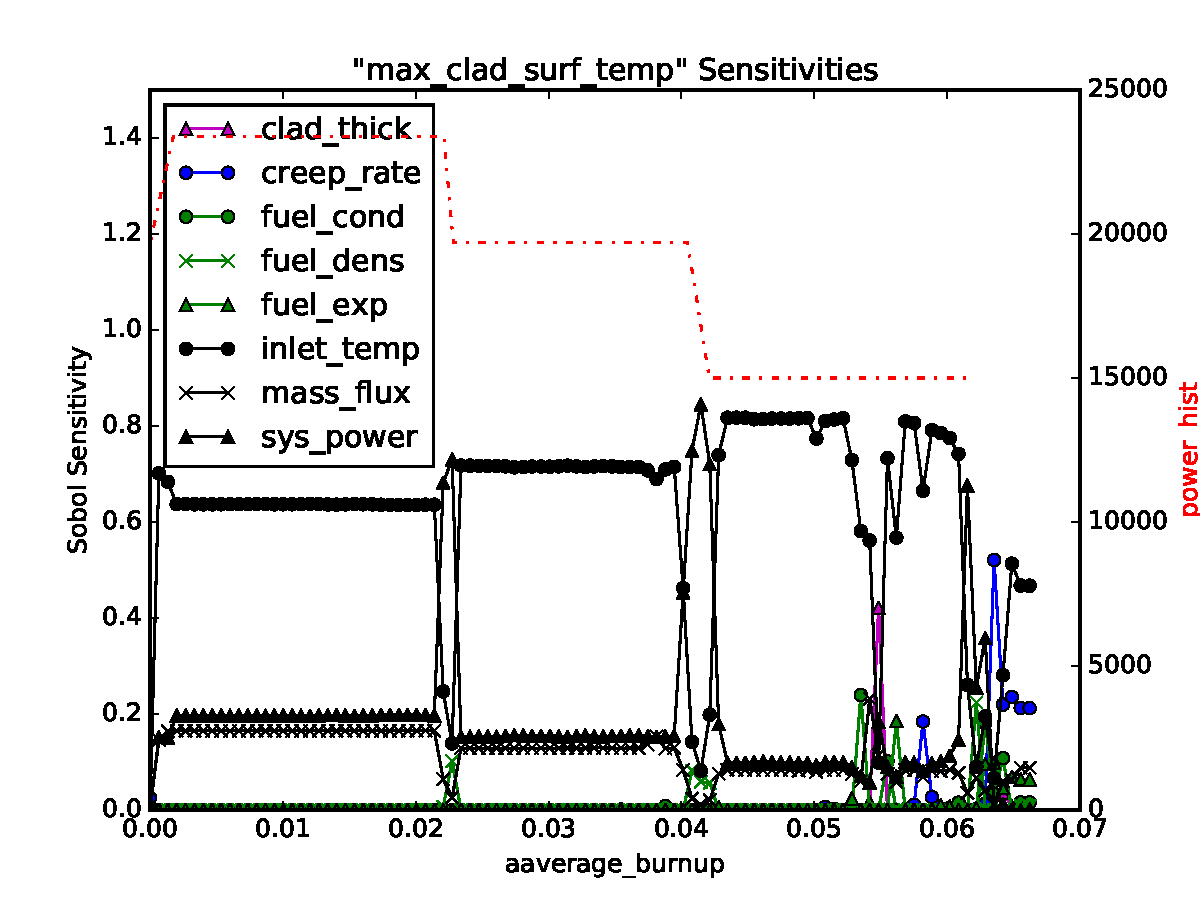
\includegraphics[width=0.7\linewidth]{oecd/sens_max_clad_surf_temp}
  \caption{Maximum Clad Surface Temperature Sensitivities}
  \label{fig:oecd clad temp}
\end{figure}
As can be seen in Figure \ref{fig:oecd clad temp}, the variance in this parameter is dominated throughout the
simulation by the variance in the inlet temperature of the moderator.  Immediately around power changes,
however, there are spikes where the variance in peak clad temperature is instead dominated for a very short
time by the system power, instead.  This is reasonable, since the inlet moderator temperature determines the
amount of heat that can be transferred out of the clad and into the moderator.  However, near changes in the
system power, and before steady-state operation is achieved, variance in the system power itself will drive
the amount of heat transferred from the fuel to the clad, and dominates the variance in the clad temperature.

In a similar fashion, we see a trade off between two less-impacting variables.  The mass flux, or the amount
of moderator passing over the cladding, and fuel density share a similar relationship as the inlet temperature
and the system power. During
steady-state operation the clad temperature is more sensitive to the mass flux, but this exchanges with fuel
density near power transients, for the same reasons as the inlet temperature and system power.

Interestingly, we see several new parameters demonstrating impact near the end of the simulation at high
burnup.  The fuel conductivity, clad thickness, fuel expansion coefficient, and creep rate all exhibit
stronger influence toward the end of life, though the inlet temperature continues to be dominant except for a
peak around 0.055 FIMA, where there is a transition in physics that emphasizes the clad thickness over other
inputs. This is likely because the peak clad temperature reaches quite low values towards the end of its life,
as the fuel produces less heat.

\subsection{Percent Fission Gas Released}
During fission events on the atomic scale in the fuel, some of the products are fission gases.  These are
often radioactive themselves and can escape the confines of the fuel and cladding more easily than pieces of
fuel, making them another design concern for mitigating contamination of the moderator.
\begin{figure}[H]
  \centering
  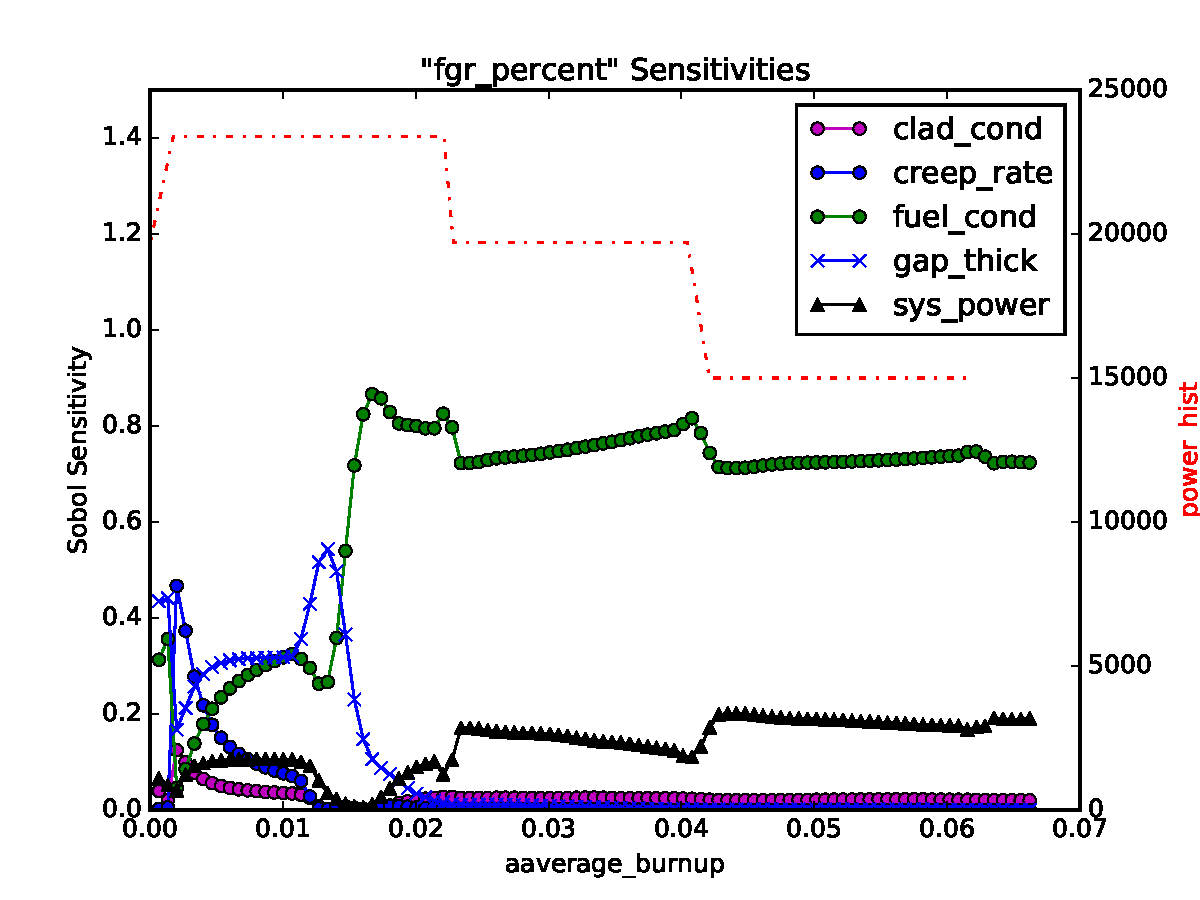
\includegraphics[width=0.7\linewidth]{oecd/sens_fgr_percent}
  \caption{Percent Fission Gas Released Sensitivities}
  \label{fig:oecd fgr}
\end{figure}
As can be seen in Figure \ref{fig:oecd fgr}, the variance in this parameter is split into two regions,
with some effects crossing between the two.  The dividing phenomenon appears to be when the fuel has expanded
through the gap to contact the cladding, which occurs around 0.015 FIMA.  Prior to this, there is an
interesting interplay between the sensitivities to gap thickness, the creep rate, and the fuel conductivity, 
with lesser impact
from the system power and clad conductivity.  Clearly the ability to remove heat effectively from the fuel has
a large impact on how likely fission gas is released.  After contact, the variance in the fuel conductivity
and system power dominate variance in the fission gas released.


\subsection{Maximum Cladding Creep Strain}
Cladding \emph{creep} describes the physics of pressurized water outside the fuel cladding pressing onto the
cladding while the cladding experiences changes in temperature.  Clad creep strain is the measure of the
strain on the cladding as a result of creep.
\begin{figure}[H]
  \centering
  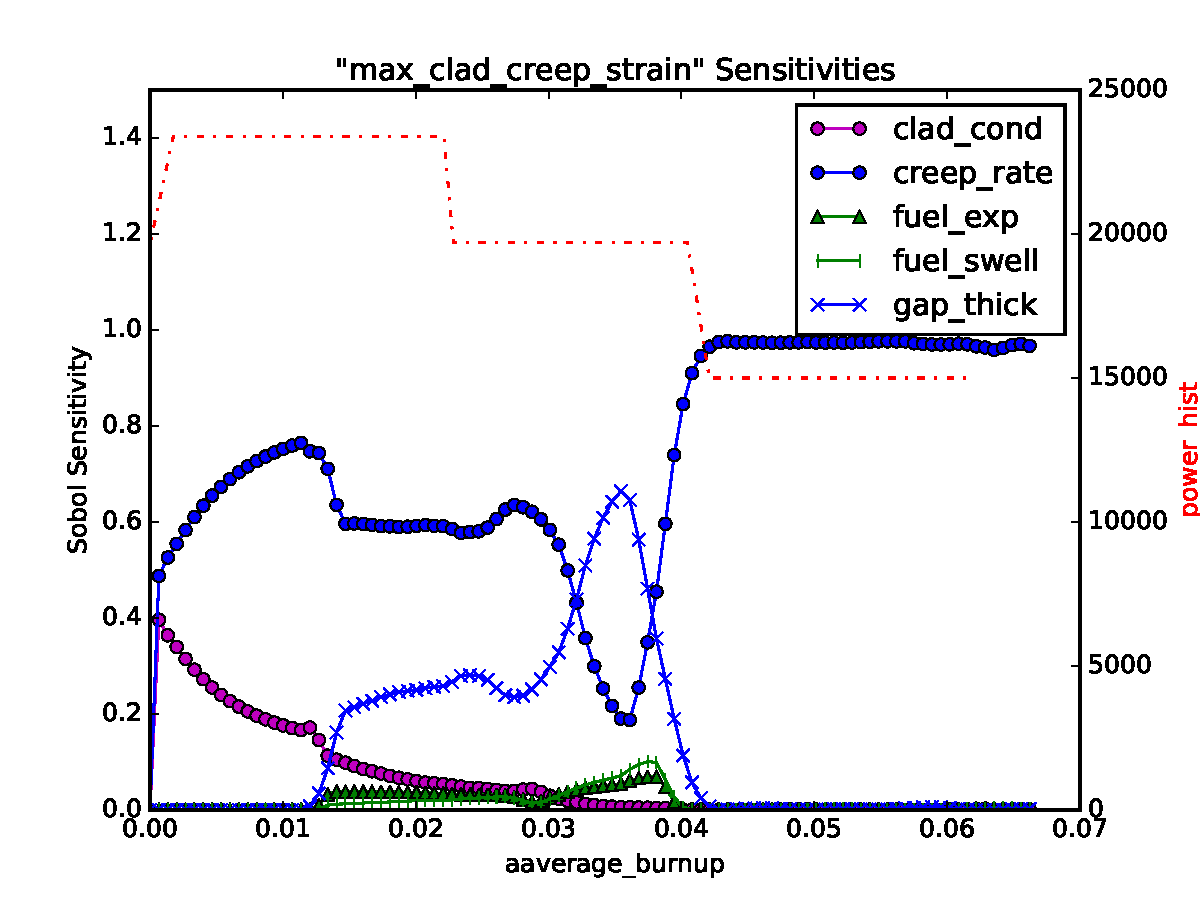
\includegraphics[width=0.7\linewidth]{oecd/sens_max_clad_creep_strain}
  \caption{Maximum Cladding Creep Strain Sensitivities}
  \label{fig:oecd strain}
\end{figure}
As can be seen in Figure \ref{fig:oecd strain}, the variance in this parameter has three distinct regions: before
fuel-clad contact, high-power contact, and low-power contact.  Nearly all the way through the simulation, the
variance in the creep strain is unsurprisingly dominated by variance in the creep rate.  Once contact is made,
however, the gap thickness plays a more important role, and grows in importance until the second drop in
power.  This is likely because the creep strain is mitigated by the expanding fuel pushing back onto the
cladding, and the size of the gap determines how early that strain begins to be relieved.

Also interestingly, the variance in the clad conductivity is initially important, but tails off as physics
besides the moderator pressure begin influencing the creep strain.  The fuel expansion and fuel swelling
parameters, which describe the fuel expansion as a result of both thermal expansion and cracking and expansion
due to fission gas buildup, are important after contact and before the second power drop, but insignificant
in the first and third sections.


\subsection{Clad Elongation}
Clad elongation measures the changing length of the clad as temperatures and pressures act on it throughout
the simulation.  As seen in Figure \ref{fig:oecd mean}, the clad tends to elongate quickly under high power,
but tails off as power diminishes.
\begin{figure}[H]
  \centering
  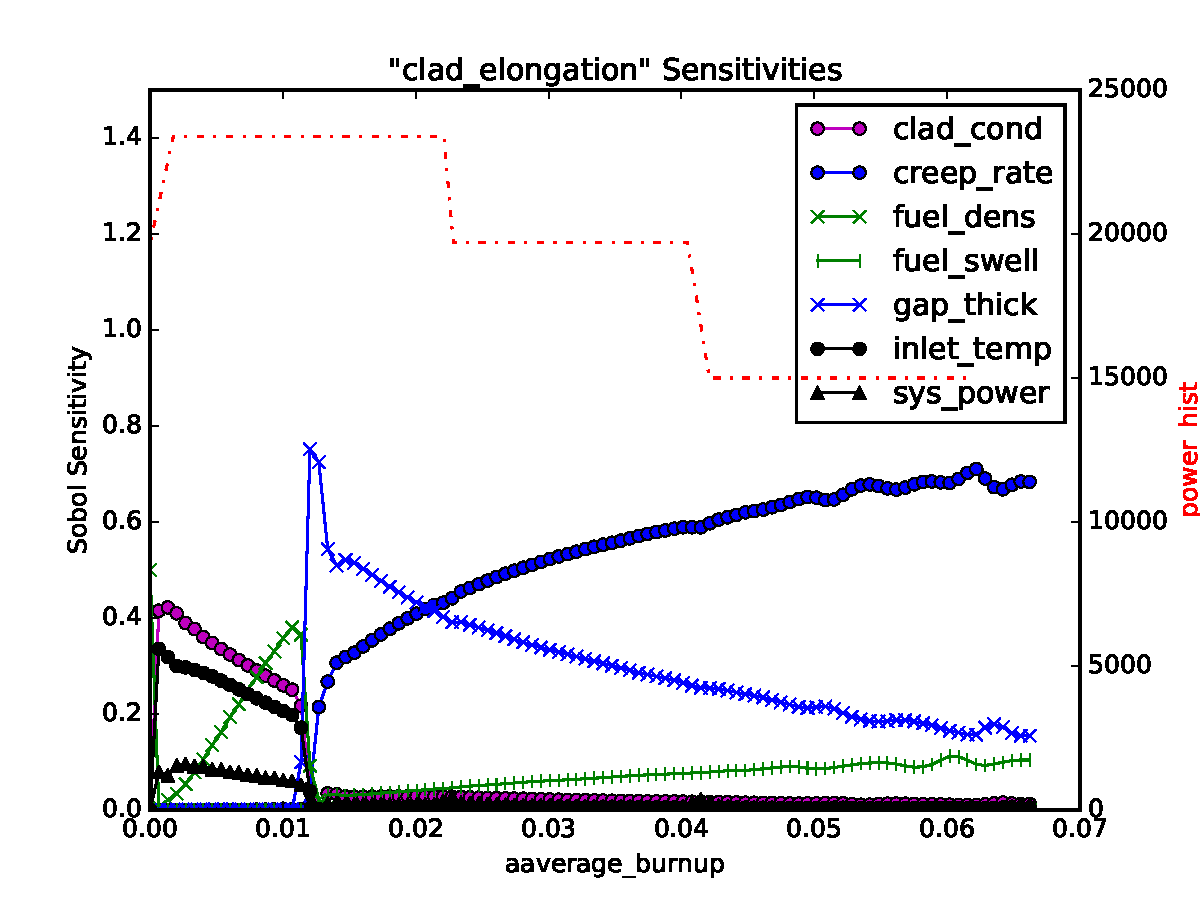
\includegraphics[width=0.7\linewidth]{oecd/sens_clad_elongation}
  \caption{Clad Elongation Sensitivities}
  \label{fig:oecd elong}
\end{figure}
As can be seen in Figure \ref{fig:oecd elong}, the variance in this parameter has two remarkably different
sets of physics, one before fuel-clad contact and one after.  Before contact, the variance in the elongation
is determined by variance in the clad conductivity, inlet temperature, and system power, with growing
importance from the fuel density.  The first three parameters all deal with the amount of heat the clad is
receiving and its ability to remove it, suggesting during this phase thermal expansion is the main source of
elongation.  As the fuel expands, however, the fuel density becomes important up until contact is made.

After contact, the elongation variance is initially determined almost solely by the gap thickness, which determines
when exactly the fuel begins to push on to the clad.  This slowly trades places with the creep rate as power
levels diminish and the expanding fuel provides less variance than the pressure of the moderator.
Interestingly, even as the gap thickness diminishes in importance, the fuel swelling parameter grows during
the power reduction, showing how after contact the gap thickness becomes less important than the swelling of
the fuel itself.



\section{Conclusion}
Time-dependent sensitivity analysis provides means to better understand uncertainty propagation throughout a transient simulation.
As physics shift throughout the simulation, so too does the sensitivity of the response to the input parameters.  If this same
simulation were performed using only static analysis on time-averaged responses, the ability to make clear decisions would be
reduced because of the lack of time-dependent information.  The addition of time-dependent analysis is quite beneficial to 
analysts considering time-dependent simulations.

